%
\section{Impact on the CE acceptance}

\begin{itemize}
\item
  two geometry options: default vs 'converter in'
\item
  for each option: 2.5 CE events, LO, perfect geometry
\end{itemize}

Distributions in Figure~\ref{figure:ce_momentum} show an impact of a 2cm wide, 100 um thin
gold converter ring on the CE acceptance. Shown there are the reconstructed CE momentum
distributions for two geometries - 'default' vs 'default plus converter ring'.

Plotted are all reconstructed tracks, no selections.

Within statistical uncertainties, the total number of the reconstructed tracks doesn't change.

Adding the converter ring reduces the number of tracks in the momentum range 103.0-105.0 MeV/c
by $\sim$ 0.2\%.

\begin{figure}[H]
  \begin{tikzpicture}
    \node[anchor=south west,inner sep=0] at (0,0.) {
      % \node[shift={(0 cm,0.cm)},inner sep=0,rotate={90}] at (0,0) {}
      % \makebox[\textwidth][c] {
        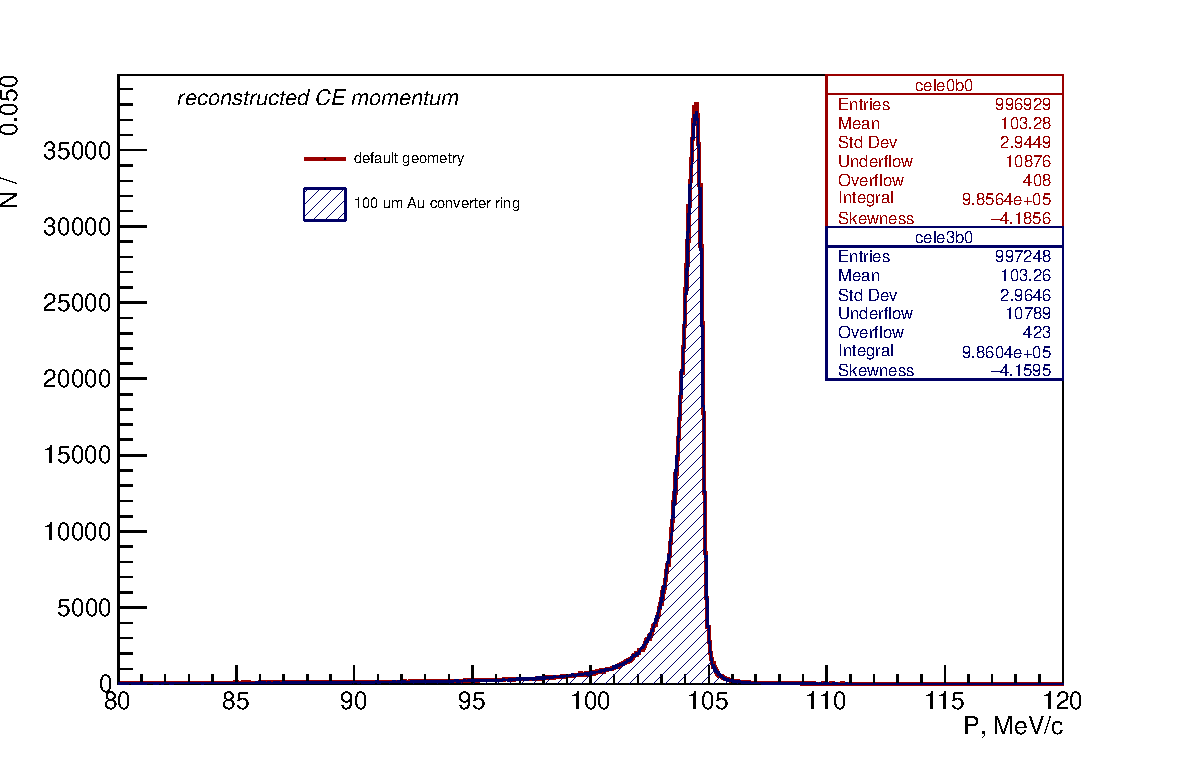
\includegraphics[width=0.54\textwidth]{pdf/figure_00051}
      % }
    };
    \node[anchor=south west,inner sep=0] at (9.8,0.) {
      % \node[shift={(0 cm,0.cm)},inner sep=0,rotate={90}] at (0,0) {}
      % \makebox[\textwidth][c] {
        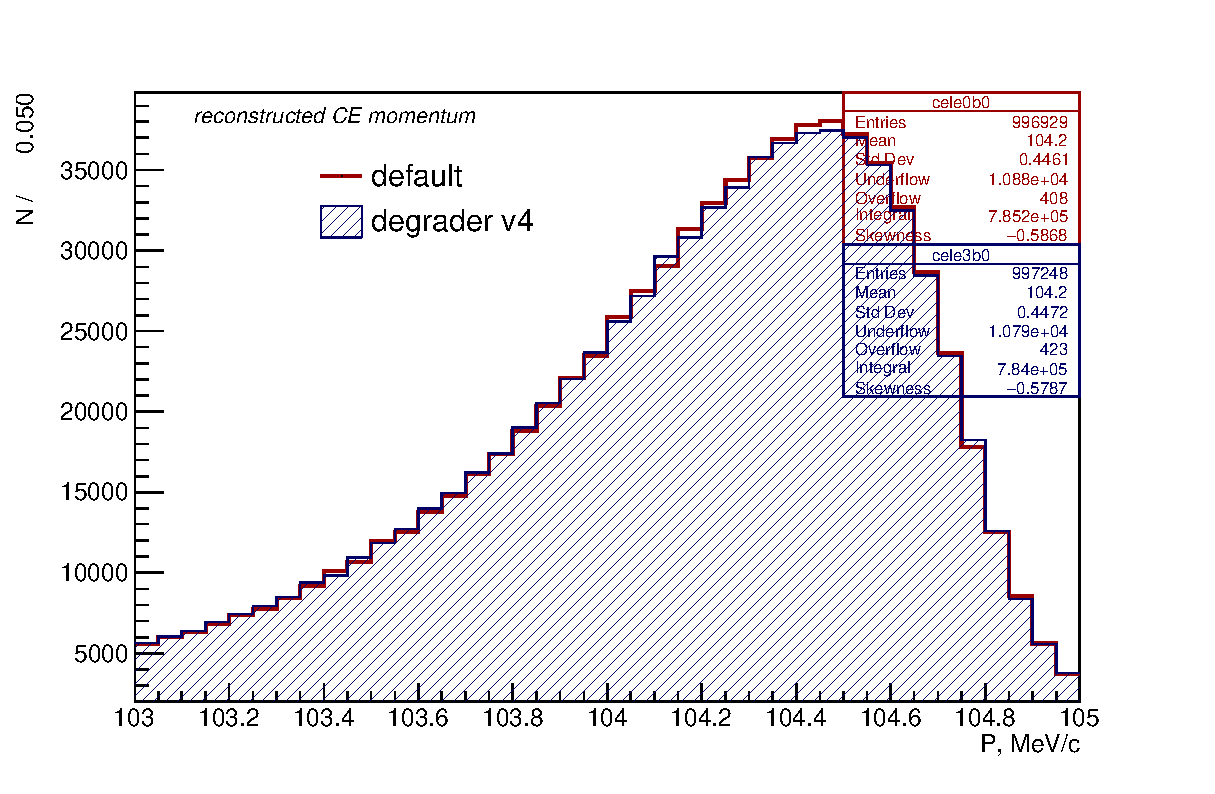
\includegraphics[width=0.54\textwidth]{pdf/figure_00052}
      % }
    };
    % \node [text width=8cm, scale=1.0] at (14.5,0.5) {$\mu_B$, expected background mean};
    % \node [text width=8cm, scale=1.0, rotate={90}] at (1.5,7.5) { $S_{D}$, ``discovery'' signal strength  };
  \end{tikzpicture}
  \caption{
    \label{figure:ce_acceptance}
    CE momentum distribution for two geometries, with an without the converter ring
  }
  \label{figure:ce_momentum}
\end{figure}


%%% Local Variables:
%%% mode: latex
%%% TeX-master: t
%%% End:
